% 投稿文章的 TeX 模板(含引用部分)
\documentclass[12pt]{article}
\usepackage{graphicx} %插入图片的宏包
\usepackage{float} %设置图片浮动位置的宏包
\usepackage{subfigure} %插入多图时用子图显示的宏包
\usepackage{amsmath,amssymb}
\usepackage{hyperref}
\usepackage[utf8]{inputenc}
\usepackage{geometry}
\geometry{a4paper, margin=1in}
\usepackage{cite} % 管理引用

\title{ZheDa DataSet in China}
\author{Name1, Name2, Name3}
\date{\today}

\begin{document}
\maketitle

\begin{abstract}
% 在此处填写摘要
\end{abstract}

\section*{Background \& Summary}
% 请在此处添加内容。例如:文献\cite{example1}中介绍了相关背景。

\section*{Methods}
\subsection*{Data collection}
% 数据采集内容

\subsection*{Data processing}
% 数据处理内容
During the data acquisition process, several files are missing, leading to gaps in the data for \emph{PQ\_nodes}, \emph{PV\_nodes}, \emph{voltage\_profile},\emph{admittance matrix} ,\emph{edges}. These missing files are recorded in a list (e.g., \texttt{missing\_files.txt}), indicating that for certain timestamps, the corresponding data is absent.

To address the issue , we utilize adjacent available data within a window of one day (or more, if needed) to complete the missing information. For the \emph{PQ\_nodes}, \emph{PV\_nodes}, and \emph{voltage\_profile}, a majority-vote strategy is applied by stacking the available data from nearby timestamps and determining the estimated value at each node based on whether the sum exceeds half the number of available samples. For the \emph{edges} field, a union of all edges from the adjacent available files is taken to reconstruct the missing edge information.

This method leverages temporal continuity by using information from proximate timestamps, ensuring that the estimation is based on relevant and recent data. The majority-vote strategy ensures robustness against outliers while the union approach for edges preserves all unique connections. As a result, the completion method provides a reliable and consistent reconstruction of missing data.

% 插入图片:PQ_nodes, PV_nodes, voltage_profile
\begin{figure}[H]
    \centering
    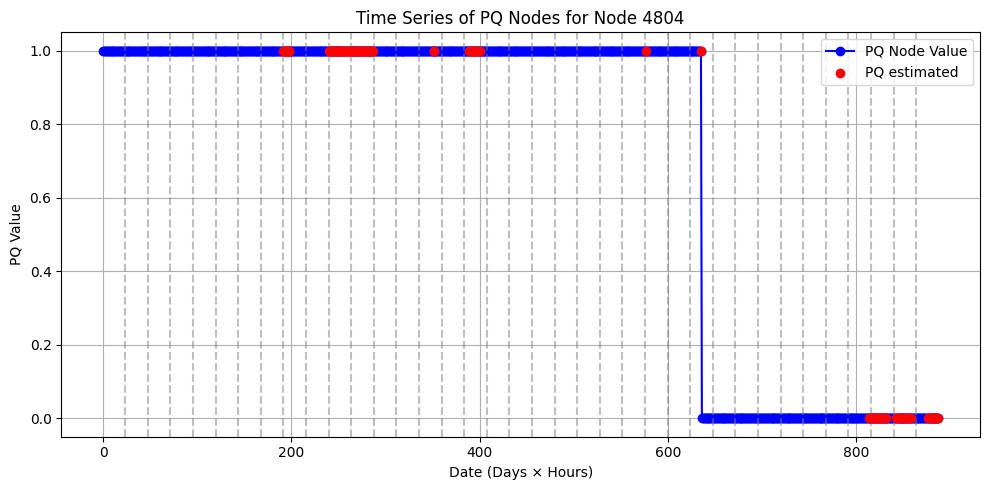
\includegraphics[width=0.7\textwidth]{picture/PQ_nodes.png}
    \caption{PQ\_nodes}
    \label{fig:PQ_nodes}
\end{figure}

\begin{figure}[H]
    \centering
    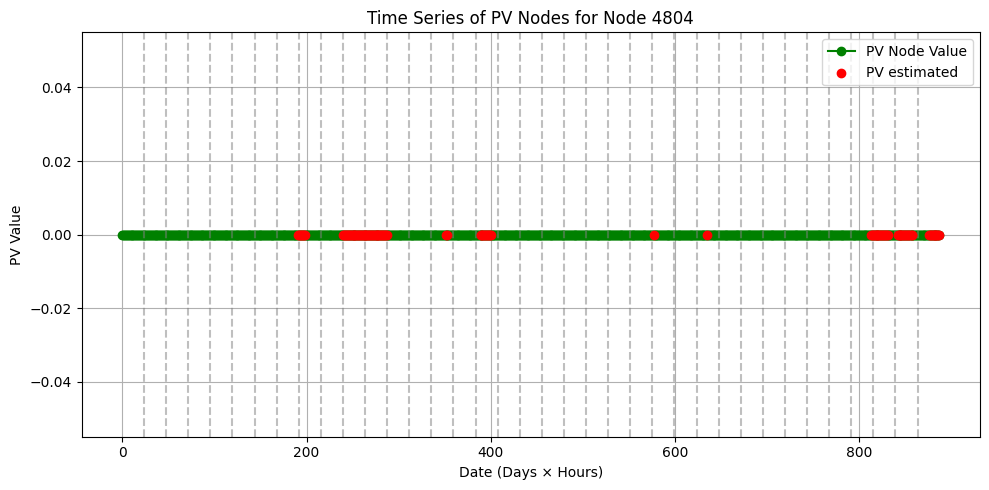
\includegraphics[width=0.7\textwidth]{picture/PV_nodes.png}
    \caption{PV\_nodes}
    \label{fig:PV_nodes}
\end{figure}

\begin{figure}[H]
    \centering
    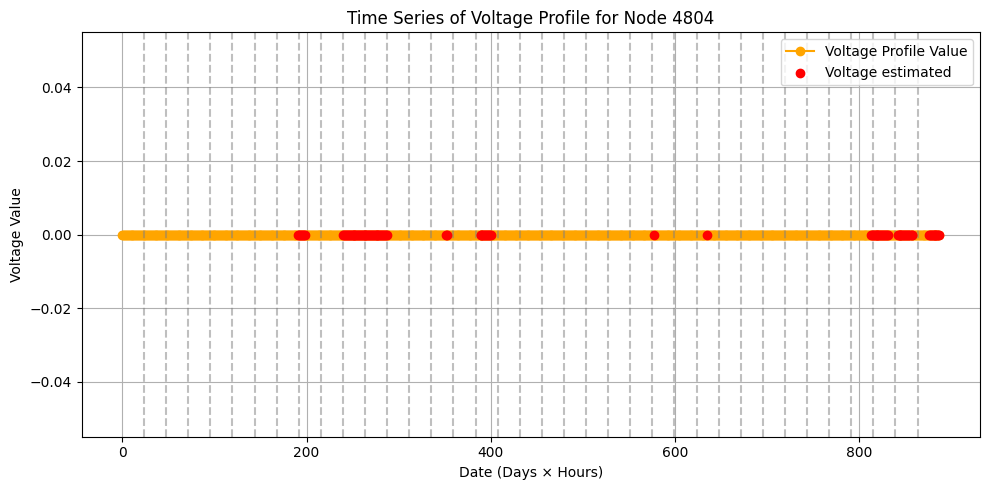
\includegraphics[width=0.7\textwidth]{picture/voltage_profile.png}
    \caption{voltage\_profile}
    \label{fig:voltage_profile}
\end{figure}

As shown in Figure~\ref{fig:PQ_nodes}, Figure~\ref{fig:PV_nodes} and Figure~\ref{fig:voltage_profile}, the respective data processing results are clearly visualized.

For the \emph{admittance matrix} field, we employ \emph{cubic spline interpolation} to estimate the missing values in the admittance matrix. Specifically, we first sort the available data by their timestamps and, for each element of the matrix, build a cubic spline model using the existing time-series data. This model is then used to interpolate the matrix values at the missing (target) timestamps.

Cubic spline interpolation provides a smooth and continuous estimation compared to linear methods. It is more capable of capturing nonlinear trends and ensures higher-order continuity, thus yielding a more accurate reconstruction of the underlying admittance properties.

Figure~\ref{fig:Avg_Magnitude} illustrates the variation in the average magnitude of the admittance matrix over time. 

\begin{figure}[H]
    \centering
    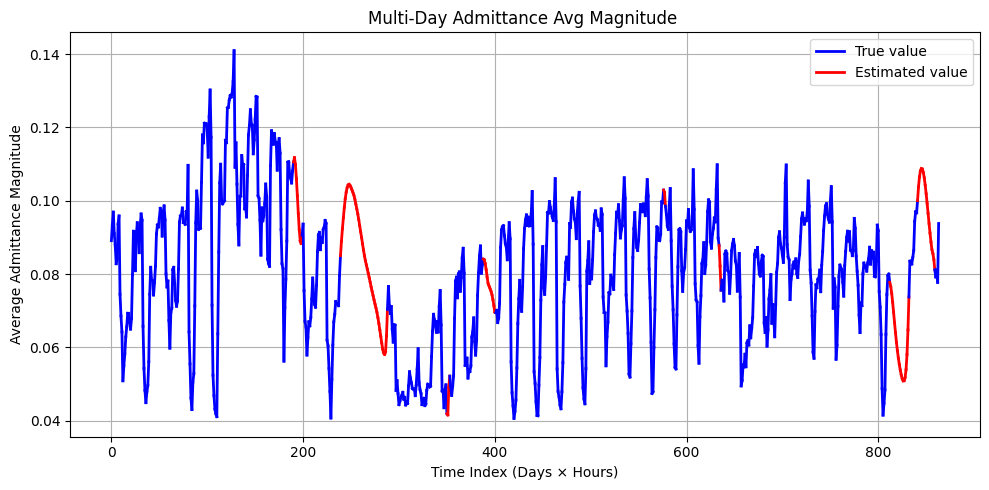
\includegraphics[width=0.7\textwidth]{picture/Avg_Magnitude.png}
    \caption{Avg\_Magnitude}
    \label{fig:Avg_Magnitude}
\end{figure}

\section*{Data Records}


% 数据记录说明
11
\section*{Technical Validation}
\subsection*{Missing value imputation}
% 缺失值填补说明

\subsection*{Fault value diagnosis}
% 故障值诊断说明

\subsection*{Correlation analysis}
% 相关性分析说明
111\cite{example1}
\subsection*{Load curve}
% 负荷曲线说明

\section*{Usage Notes}
% 使用说明

\section*{Acknowledgements}
% 致谢内容

\section*{References}
% 请在此处插入引用,可以采用 BibTeX 或手动添加参考文献。
\bibliographystyle{unsrt}  % 可选 plain、alpha、abbrv 等格式
\bibliography{references}  % 请确保有一个名为 references.bib 的 BibTeX 数据库文件


\end{document}
